\documentclass[a4paper, 12pt]{article} % добавить leqno в [] для нумерации слева
\usepackage[a4paper,top=1.3cm,bottom=2cm,left=1cm,right=1cm,marginparwidth=0.75cm]{geometry}

\usepackage[warn]{mathtext}
\usepackage[T2A]{fontenc}
\usepackage[utf8]{inputenc} 
\usepackage[english, russian]{babel}

\usepackage{tikz}
\usepackage{pgfplots}

\usepackage{ upgreek }
\usepackage[table,xcdraw]{xcolor}

\usepackage{indentfirst} %tabutation

\usepackage{amsmath, amsfonts, amssymb, amsthm, mathtools, mathtext} 

\usepackage{graphicx}

\usepackage{wrapfig}
\usepackage{tabularx}

\usepackage{graphicx}%Вставка картинок правильная
\usepackage{float}%"Плавающие" картинки
\usepackage{wrapfig}% Обтекание фигур (таблиц, картинок и прочего)

%%% Дополнительная работа с математикой
\usepackage{amsmath,amsfonts,amssymb,amsthm,mathtools} % AMS





%%% Заголовок
\title{Лабораторная работа №3.7.1}
\date{\today}

\begin{document}

\begin{center}
	{\large МФТИ ФРКТ}
\end{center}

{\huge
	\begin{center}
		{\bf Лабораторная работа 3.7.1}\\
		 Скин-эффект в полом цилиндре
	\end{center}
}
\begin{center}
	Владимир Трунов, Андрей Строчук
\end{center}

\section*{Введение}

\textbf{Цель работы:}
	исследование проникновения переменного магнитного потока в медный полый цилиндр.

\medskip

\textbf{В работе используются:} генератор звуковой частоты, соленоид, намотанный на полый цилиндрический каркас из диэлектрика, медный экран в виде трубки, измерительная катушка, амперметр, вольтметр, осциллограф.

\medskip




\section{Общая теория скин-эффекта}
\begin{wrapfigure}{l}{0.2\textwidth}
		\vspace{-20pt}
		\begin{center}
			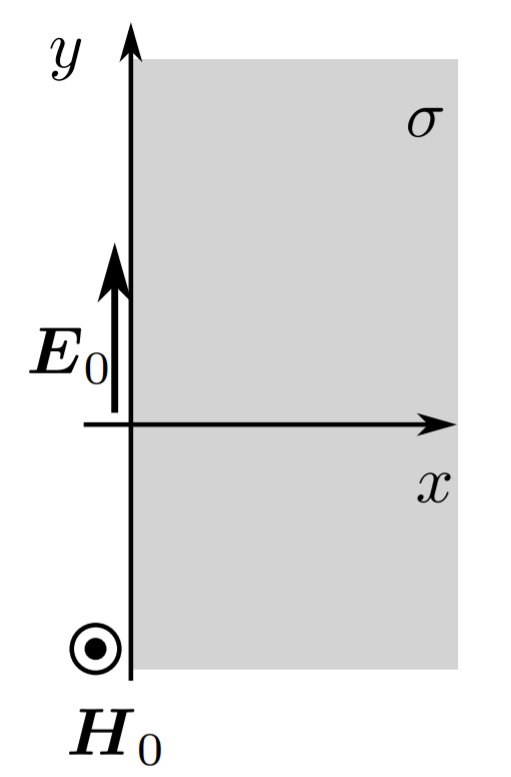
\includegraphics[height=0.2\textheight]{Skin1.png}
		\end{center}
		\vspace{-20pt}
		\caption{Скин-эффект в плоской геометрии}
		\vspace{20pt}
	\end{wrapfigure}

	Рассмотрим квазистационарное поле внутри проводящей среды в простейшем плоском случае. Пусть вектор $\boldsymbol{H}$ направлен всюду вдоль оси $z$ и зависит только от координаты $x$, то есть $H_x = H_y \equiv 0$.
	
	
	\noindent Из уравнений Максвелла следует равенство:
	
	\begin{equation}
		\nabla^2\boldsymbol{H} = \sigma\mu\mu_0\dfrac{\partial\boldsymbol{H}}{\partial t}.
	\end{equation}
	
	\noindent В нашем случае оно примет вид:
	
	\begin{equation}
		\dfrac{\partial^2 H_z}{\partial x^2} = \sigma\mu\mu_0 \dfrac{\partial H_z}{\partial t}.
	\end{equation} 

	\noindent Пусть полупространство $x > 0$ заполнено проводящей средой с проводимостью $\sigma$, а на границе $x = 0$ задано магнитное поле, изменяющееся по гармоническому закону: $H_z = H_0 e^{i\omega t}$. Будем искать решение уравнения выше также в виде гармонической функции: $H_z(x, t) = H(x)e^{i\omega t}$.
	
	\noindent После подстановки в уравнение получим:
	
	\begin{equation}
		\dfrac{d^2 H}{dx^2} = i\omega\sigma\mu\mu_0H.
		\label{H_diff}
	\end{equation}

	\noindent Как известно из теории линейных дифференциальных уравнений,
	решение нужно искать в виде: $H(x) = H_0 e^{k x}$. Подставляя, получим,
	что уравнение имеет нетривиальные решения такого вида при $k^2 = i\omega\sigma\mu\mu_0$. Откуда получаем:
	
	\begin{equation}
		k = \pm \dfrac{1+i}{\sqrt{2}}\sqrt{\omega\sigma\mu\mu_0}.
	\end{equation}

	\noindent Для полубесконечной среды $(z > 0)$ физический смысл имеет только решение со знаком минус, соответствующее стремлению к нулю амплитуды поля при $z \rightarrow \infty$. Окончательное решение уравнения:
	
	\begin{equation}
		H_z(x, t) = H_0e^{-x/\delta}e^{i(\omega t - x/\delta)},
	\end{equation}

	\noindent где $\delta = \sqrt{\dfrac{2}{\omega\sigma\mu\mu_0}} = \dfrac{1}{\sqrt{\pi f \sigma\mu\mu_0}}$ - \textbf{глубина проникновения} поля, или \textbf{скиновая} глубина.
	


\section{Специфика работы}


В работе изучается скин-эффект в длинном тонкостенном медном цилиндре, помещённом внутрь соленоида, поэтому $\mu \approx 1$ с хорошей точностью.
	
	Если выполнено условие $h \ll a$, то для описания поля внутри стенки можно ограничиться одномерным приближением. После решения уравнения (\ref{H_diff}) и подстановки граничных условий $H(0) = H_0$, $H(h) = H_1$ приходим к главной формуле всей работы:
	
	\begin{equation}
		H_{1} = \dfrac{H_0}{\frac{1}{2}ak \sh{k h} + \ch{k h}}
	\end{equation}

	Разобьем на предельные случаи.
	
	\begin{enumerate}
		\item \textbf{Малые частоты.}
			Имеем $\delta \gg h$, откуда $|kh| \ll 1$, значит $\ch kh \approx 1, \sh kh \approx kh$, и тогда:
			
			\begin{equation}
				H_1 \approx \dfrac{H_0}{1 + i\frac{ah}{\delta^2}}.
			\end{equation}
		
			Следовательно для отношения модулей получаем:
			\begin{equation}
				\dfrac{|H_1|}{|H_0|} = \dfrac{1}{\sqrt{1+ \left(\frac{ah}{\delta^2}\right)^2}} = \dfrac{1}{\sqrt{1 + \frac{1}{4}\left(ah\sigma\mu_0\omega\right)^2}} = \dfrac{1}{\sqrt{1 + \left(ah\pi f\sigma\mu_0\right)^2}}.
			\end{equation}
		
		 	А фаза $H_1$ отстает от фазы $H_0$ на $\psi = \arctg\left(\dfrac{ah}{\delta^2}\right)$.
		 	
		 \item \textbf{Большие частоты.} 
		 	Ситуация обратная -- $\delta \ll h$. Тогда $|kh| \gg 1$ и 	$|ka| \gg 1$, откуда $\sh kh \approx \ch kh \approx \dfrac{1}{2}e^{kh}$, и тогда:
		 
		 	\Large
			\begin{equation}
			 	\frac{H_1}{H_0} = \frac{4}{ka}e^{-kh} = \frac{2\sqrt{2}\delta}{a}e^{-\frac{h}{\delta}}e^{-i\left(\frac{\pi}{4} + \frac{h}{\delta}\right)}.
			 	\label{high}
			\end{equation}
	\end{enumerate}
	

	
	Как видно из формулы (\ref{high}), в этом пределе поле внутри цилиндра по модулю в $\frac{2\sqrt{2}\delta}{a}e^{-h/\delta}$ раз меньше, чем снаружи, и, кроме того, запаздывает по фазе на:
	
	\begin{equation}
		\psi = \frac{\pi}{4} + \frac{h}{\delta} = \frac{\pi}{4} + h\sqrt{\pi f \sigma\mu_0}.
		\label{freq}
	\end{equation}

\section{Экспериментальная установка}
	\begin{figure}[h!]
		\centering
		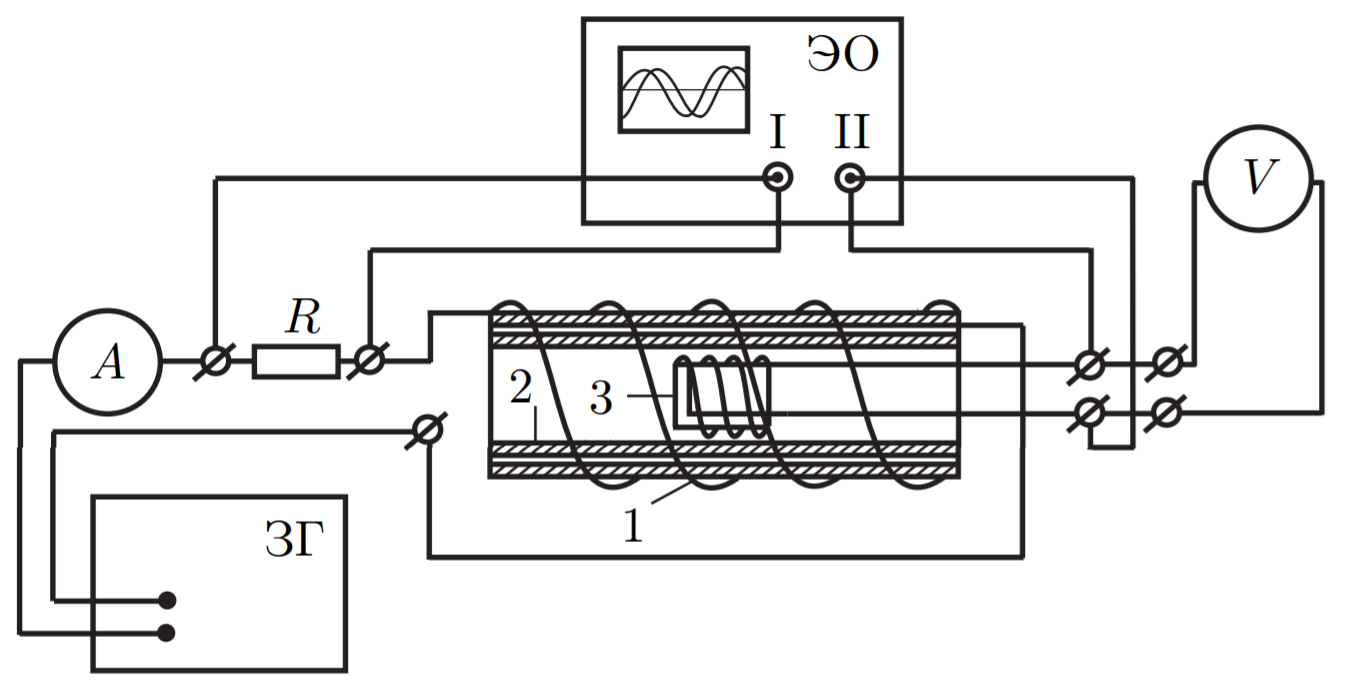
\includegraphics[scale=0.5]{Scheme.png}
		\caption{Экспериментальная установка для изучения скин-эффекта}
	\end{figure}

	Схема экспериментальной установки для исследования проникновения переменного магнитного поля в медный полый цилиндр изображена на рис. 3. Переменное магнитное поле создаётся с помощью соленоида, намотанного на полый цилиндрический каркас 1 из поливинилхлорида, который подключается к генератору звуковой частоты. Внутри соленоида расположен медный цилиндрический экран 2. Для измерения магнитного поля внутри экрана используется измерительная катушка 3.
	
	С помощью вольтметра $V$ измеряется действующее значение ЭДС индукции, которая возникает в измерительной катушке, находящейся в переменном магнитном поле $H_1 e^{i\omega t}$. Комплексная амплитуда ЭДС индукции в измерительной катушке равна 
	\begin{equation*}
		\widehat{U} = -SN \frac{d\widehat{B_1}(t)}{dt} = -i\omega\mu_0 SN H_1 e^{i\omega t}.
	\end{equation*}
	
	Показания вольтметра, измеряющего это напряжение, будут тогда, соответственно, равны:
	\begin{equation*}
		U = \frac{SN\omega}{\sqrt{2}}\mu_0 |H_1|.
	\end{equation*}

	Видно, что модуль амплитуды магнитного поля внутри экрана $|H_1|$ пропорционален $U$ и обратно пропорционален частоте сигнала $f$:
	\begin{equation*}
		|H_1| \propto \frac{U}{f}.
	\end{equation*}

	При этом поле вне экрана $|H_0|$ пропорционально току $I$ в цепи соленоида, измеряемому амперметром $A$:
	\begin{equation*}
		|H_0| \propto I.
	\end{equation*} 

	Следовательно:
	\begin{equation}
		\frac{|H_1|}{|H_0|} = \text{const} \cdot \frac{U}{fI}
	\end{equation}

	Таким образом, отношение амплитуд магнитных полей снаружи и
	вне экрана (коэффициент ослабления) может быть измерено по отношению $\frac{U}{fI}$ при разных частотах, а неизвестная константа в соотношении может быть определена по измерениям при малых частотах.

	\section {Определение проводимости материала экрана}
	В установке в качестве экрана используется медная труба промышленного производства. Технология изготовления труб оказывает заметное влияние на электропроводимость. Из-за наличия примесей проводимость меди трубы в данной работе отличается от табличного значения в меньшую сторону. Для определения $\sigma$ экрана будем использовать частотную зависимость (\ref{freq}) фазового сдвига между магнитными полями внутри и вне экрана при высоких частотах. Как видно из выражения (\ref{freq}), в области больших частот $f \gg \frac{1}{h^2 \pi \sigma\mu_0}$ зависимость $\psi(\sqrt{f})$ аппроксимируется прямой, проходящей через точку $\psi(0) = \frac{\pi}{4}$. По наклону этой прямой можно вычислить проводимость материала экрана.
	
	\section *{Ход работы}
	
	1. При $ \nu_{h} = 2263.5 Гц 	$ толщина стенок h равна скиновой глубине $\delta$.
	
    2. Получим зависимость $\xi = U/I\nu$ при малых частотах от $0,01\nu_h$ до $0.05\nu_h$.
    
    
    
	\centering
	    \begin{table}[!ht]
            \centering
            \begin{tabular}{|l|l|l|l|}
             \hline
            U, V & I, mA & $\nu$, Hz & $\xi$ \\ \hline
            0,0052 & 21,84 & 20 & 0,011904762 \\ \hline
            0,0068 & 21,818 & 25 & 0,012466771 \\ \hline
            0,0083 & 21,78 & 30 & 0,012702785 \\ \hline
            0,0097 & 21,724 & 35 & 0,012757451 \\ \hline
            0,0111 & 21,656 & 40 & 0,012814001 \\ \hline
            0,0124 & 21,573 & 45 & 0,012773168 \\ \hline
            0,0137 & 21,492 & 50 & 0,01274893 \\ \hline
            0,015 & 21,397 & 55 & 0,012746052 \\ \hline
            0,0173 & 21,197 & 65 & 0,012556204 \\ \hline
            0,0194 & 20,985 & 75 & 0,012326265 \\ \hline
            0,0214 & 20,769 & 85 & 0,012122139 \\ \hline
            0,023 & 20,551 & 95 & 0,011780705 \\ \hline
            0,0246 & 20,338 & 105 & 0,011519604 \\ \hline
            \end{tabular}
    \end{table}

\medskip	

	4. Исследовали зависимость величины $\xi$ от фазового сдвига $\psi$ при малых частотах от $0,05\nu_h$ до $0.5\nu_h$
	
	
	5. Исследовали зависимость величины $\xi$ от фазового сдвига $\psi$ при высоких частотах от $0,5\nu_h$ до $15\nu_h$
	
	6. Исследуем зависимость индуктивности катушки L от частоты $\nu$ в диапазоне от $\nu_{min} = 40 Гц$ до $1.5\nu_h$.
	
	\section *{Обработка данных}
	1. Построим график зависимости $f(\nu^2)$ от $1/\xi^2$.
		\begin{figure}
		\centering
		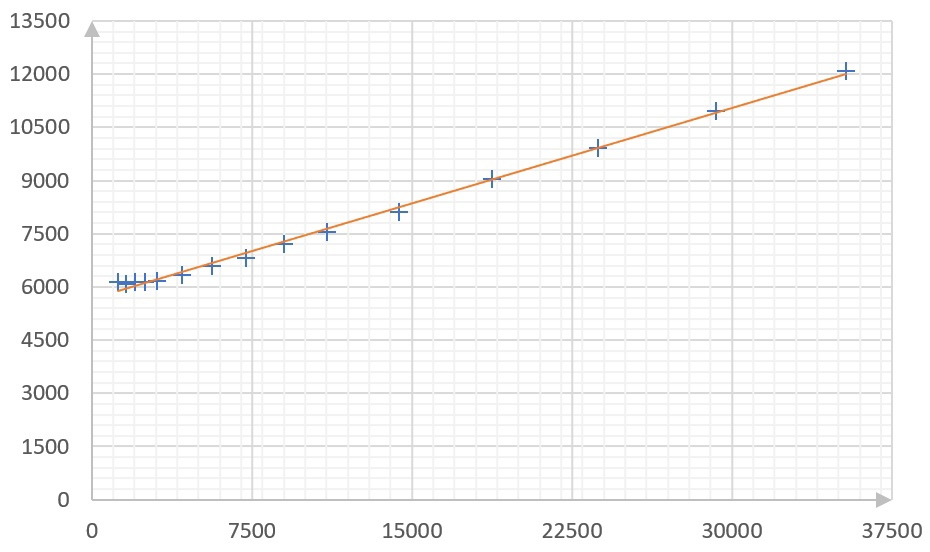
\includegraphics[width = 18cm]{graph1.jpg}
		\caption{график зависимости $f(\nu^2)$ от $1/\xi^2$}
	\end{figure}
	
	Получили линейную зависимость. Теперь с помощью экстраполяции найдем $\xi_0$ - коэффициент пропорциональности между $\xi$ и коэффициентом ослабления магнитного поля $|H_1|/|H_0|$.
	\begin{equation*}
		\xi_0  = 13.29 \pm 0.02 мОм * с
	\end{equation*}
	
	Рассчитаем проводимость меди из формулы:
	\begin{equation}
				\dfrac{|H_1|}{|H_0|} = \dfrac{1}{\sqrt{1+ \left(\frac{ah}{\delta^2}\right)^2}} = \dfrac{1}{\sqrt{1 + \frac{1}{4}\left(ah\sigma\mu_0\omega\right)^2}} = \dfrac{1}{\sqrt{1 + \left(ah\pi f\sigma\mu_0\right)^2}}.
			\end{equation}
	\begin{equation*}
\sigma  = (41.3 \pm 0.7)\times 10^6 \text{ Ом}^{-1}.
	\end{equation*}


2. Построим график зависимости f($\nu$) =  tg$\psi$. 
		\begin{figure}
		\centering
		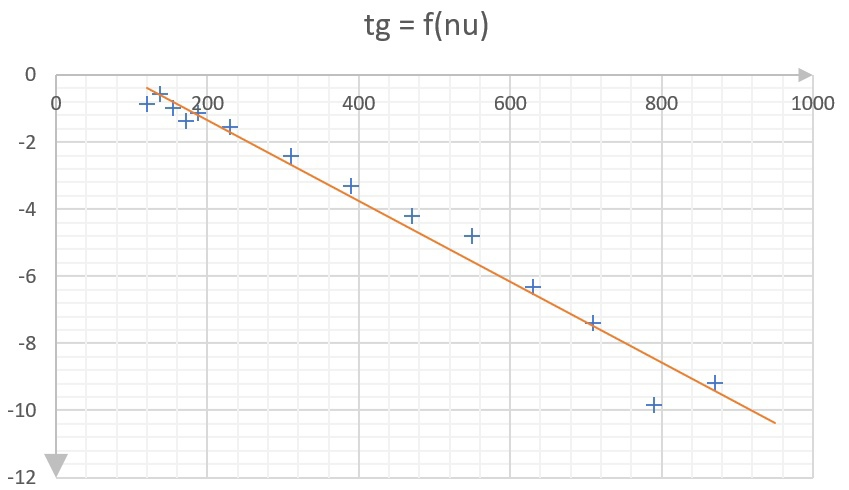
\includegraphics[width = 15cm]{graph2.jpg}
		\caption{график зависимости f($\nu$) = tg$\psi$ }
	\end{figure}
	
По наклону прямой определяем коэффициент проводимости $\sigma$
	\begin{equation*}
\sigma = 45.4 \pm 0.6 * 10^6 Ом^{-1}
	\end{equation*}
	
3. Построим график частотной зависимости фазового сдвига $f(\sqrt{\nu}) = \psi - \pi/4$

		\begin{figure}
		\centering
		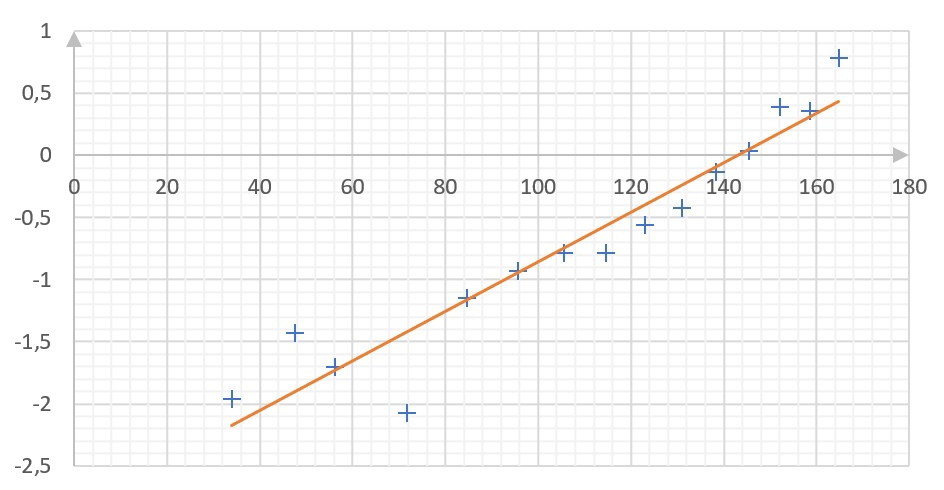
\includegraphics[width = 15cm]{graph3.jpg}
		\caption{график зависимости $f(\sqrt{\nu}) = \psi - \pi/4$}
	\end{figure}
	
По наклону касательной определим коэффициент проводимости $\sigma$ из формулы:
	\begin{equation*}
\psi = \pi/4 + h\sqrt{\frac{\omega\sigma\mu_0}{2}}
	\end{equation*}

	\begin{equation*}
\sigma = 44.8 \pm 0.7 * 10^6 Ом^{-1}
	\end{equation*}	
	
4. Построим график зависимости индуктивности катушки от частоты L($\nu$). Определим максимальное и минимальное значения индуктивности $L_{min}$ и $L_{max}$.

		\begin{figure}
		\centering
		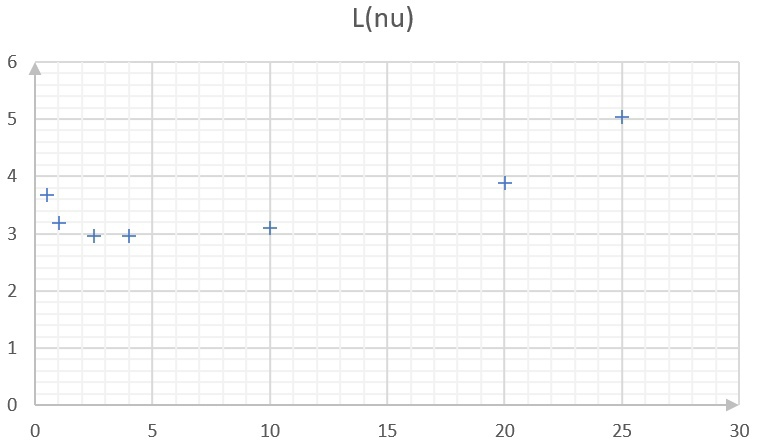
\includegraphics[width = 15cm]{graph4.jpg}
		\caption{график зависимости $L(\nu)$}
	\end{figure}	

Построим теперь график зависимости $(L_{max}-L_{min})/(L-L_{min})$ от $\nu^2$. 

		\begin{figure}
		\centering
		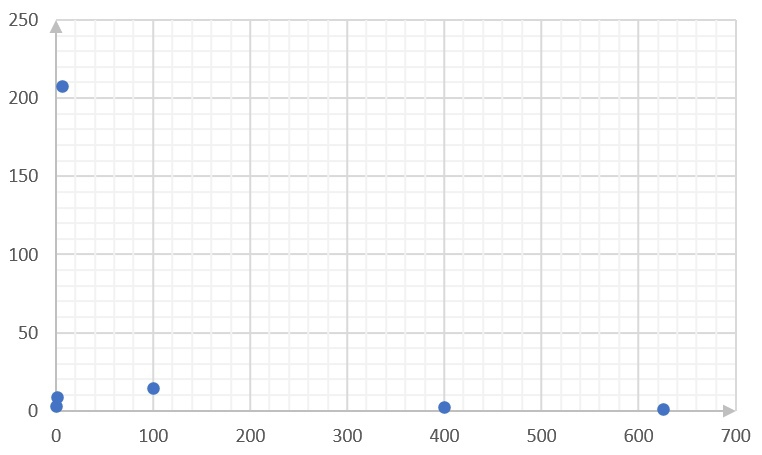
\includegraphics[width = 18cm]{graph5.jpg}
		\caption{график зависимости $(L_{max}-L)/(L-L_{min})$ от $\nu^2$}
	\end{figure}	
	\begin{equation*}
\frac{L_{max}-L}{L-L_{min}} = \pi^2a^2h^2\mu_0^2\sigma^2\nu^2
\end{equation*}	
	
5. Сведем результаты в таблицу:
\begin{table}[h!]
 \begin{center}
\begin{tabular}{|c|c|c|с|}
\hline

$\sigma_1$, $10^6 Ом^-1$  & $\sigma_2$, $10^6 Ом^-1$ & $\sigma_3$, $10^6 Ом^-1$ & $\sigma_{teor}$, $10^6 Ом^-1$ & \\ \hline
$41.3 \pm 0.7$      & $45.4\pm0.6$     & $44.8\pm0.7$ &  $55$ & \\ \hline
\end{tabular}
 \end{center}
\end{table}

В результате полученные данные совпадают с теоретическими в пределах 15%.
\fi	
\section{Вывод}
В ходе работы была получена проводимость материала цилиндра 3 способами, и результат почти совпал с теорией. Различия данных связаны со способом изготовления образца и со способом проведения измерений. 
	
\end{document}